% 	What did before starting to program. 
% 	Software engineering planning etc.
% *! Show that I understood the task and analysed it
% *! Good introduction to technical background, coherent discussion and sensible planning
% * Requirements analysis
% * Cite any new programming languages and systems which had to be learnt
% * Mention complicated theories or algorithms which required understanding

% ************
% Should have: 
% 	intro
% 	content
% 	summary
% ************

% Allowed roughly 1200 words
\chapter{Preparation}
% How did I prepare
In this chapter we will look at what considerations dictated the design choices made, why I chose Erlang as the language of implementation and how software engineering principles played a role in the successful implementation of my project.

\section{Requirements analysis}
% Requirements
% Fit into into existing services? (webservice)
% Ease of integration
My goal was to write a very particular kind of search engine, a search engine which in the end would work very much like a distributed oversized address book.
Directory services solving more or less the same problem already exist, but there are several benefits in making such a system distributed: as soon as there are more than one party contributing nodes to the distributed network, there will be no single entity owning all the data, nor any single entity having to foot the bill for running the service. Another benefit of well designed distributed systems is that they scale horizontally rather than vertically, meaning you can increase the system's performance by adding more cheap nodes run on commodity hardware, rather than buy new and more powerful machines to replace your existing ones.

The idea of not having a central authority with ownership over the data resonates especially well with independent distributed online social networks, most of which where inspired by the idea of allowing their users to themselves maintain ownership of their data and have fine grained control over what is made visible to the world at large.

Having established a distributed system was desirable, I needed to build it in such a way that nodes in the search engine could easily be hosted by independent providers of distributed online social networks. Not only would the search engine have to be easy to install and run, but it should also be easy to integrate into a wide variety of different services, all built by different teams. The search engine would also need to handle nodes joining and leaving without interruption to the service.
Handling high node churn in distributed environments without sacrificing reliability and speed is what Distributed Hash Tables are designed for. I therefore decided I wanted to use Distributed Hash Tables as the back end data store for my search engine.

From experience I know that web developers find it convenient to integrate services that expose an HTTP interface, so to meet the requirement of easy integration, I decided my search engine would expose its functionality through a HTTP based API and that the data would be sent as JSON (JavaScript Object Notation) for easy manipulation and consumption.

Both search engines and address books today provide predictive search where results show as you type, and often also fuzzy matching allowing for partially misspelled names. A search engine like the one I wanted to build, would never become popular if it did not provide the same. I therefore decided from the beginning that I wanted to include my proposed project extension of fuzzy searches.

\section{Underlying theory}
% Read through different DHT's
% Decided on three
% Cut down to two, why?
% Benefits and drawbacks of DHTs
Distributed Hash Tables are key-value stores that store data under particular keys, and given a key will return the data stored under it if it exists.
What makes Distributed Hash Tables different from regular hash tables, or dictionaries as they are called in some languages, is that the data is not stored on a single machine, but split up across a network of machines.

There are quite a few well known Distributed Hash Tables. After initial research I decided to implement and compare Chord, Pastry and Kademilia, but quickly realized Kademilia differs from Chord in ways similar to what Pastry already does, and decided to drop it from my implementation, giving me the added benefit of more time along my projects critical path that could be spent on a more thorough evaluation of the relative performance of Chord and Pastry.

\mbox{}

Distributed Hash Tables are key-value stores. In other words; unless you know the specific key under which a data item is stored, you will not be able to find it by other means than by doing a linear search through the system.

Having established that I wanted to support predictive search, and fuzzy searches where you should be allowed to misspell the name of the person you are trying to find, I had to come up with a mapping scheme that allowed me to predict the correct keys with insufficient data. 
Schemes looking up keywords in inverse indexes through flooding and random walks on top of structured and unstructured peer to peer networks have been proposed \cite{myths}, but do not give performance in the sub-second latency range that I require in order to provide predictive search.

I came up with the following solution:

Just like in a regular address book I store records containing all the information a user wants to disclose to the network. These \emph{profile records}, stored under a key created by hashing the whole profile record data structure, would include the user's full name, a link to the user's profile page hosted by his or her distributed online social network provider and preferably the address of a profile image that could be displayed alongside the search results.

In order to to find a profile record given incomplete or misspelled names, I also store \emph{link records}. A link record contains the user's full name and the key of the full profile record, but are stored under keys generated by hashing fragments of a user's name. 

I decided to generate link records separately for each of a user's names, and additionally generate a link record for each additional three characters in a user's name. A person with the name \emph{Abcdefghijk} would get a link record for the first three characters of his name, \emph{abc}, a link record created by adding the next the characters, \emph{abcdef}, another link record adding the subsequent three characters, \emph{abcdefghi}, and finally a link record for the whole name, \emph{abcdefghijk}.
As can be seen in figure \ref{figLinkRecord}, my surname \emph{Eide} would result in link records for \emph{eid} and \emph{eide} while my first name \emph{Sebastian} would result in link records for \emph{seb}, \emph{sebast} and \emph{sebastian}.

% How link records are generated
\begin{figure}[!htb]
\begin{center}
	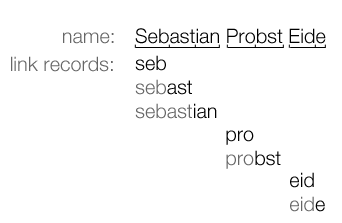
\includegraphics[width=0.6\linewidth]{illustrations/LinkRecords.png}
  \caption{Names are split into name fragments used to generate keys for link records. The slightly darker coloured parts of the link record names indicate the additional three characters added compared to the previous link record name fragment.}
  \label{figLinkRecord}
\end{center}
\end{figure}

When searching for a person the search system looks up \emph{link records} while the user types. Since \emph{link records} contain the full name of the person whose \emph{profile record} they point to, the search system can try to find out which of the possible \emph{profile records} the user is looking for by looking at the relative frequency at which the different \emph{profile records} are being linked to by the \emph{link records} downloaded. It can then download the highest ranked \emph{profile records} and display them as search results to the user while he or she is still completing the search query.

There is an overhead both in terms of storage and lookup cost associated with this approach that I will try to classify and evaluate in the evaluation chapter.

\section{Language and tools used}
%     Learned Erlang
%       Got to know standard libraries and frameworks (OTP)
%       webmachine
%       rebar
%       how to do testing
Wanting to build a highly fault tolerant and distributed system with soft real-time requirements, I decided to use the programming language Erlang.

Erlang, while a language I had never previously used, was created exactly with these requirements in mind. Its standard libraries include frameworks for building hierarchies of process supervisors that ensure processes are restarted if they terminate prematurely or become unresponsive, and Erlang also nicely abstracts away inter process communication and encourages immutable state, making problems classical programming languages have with efficient concurrency and shared memory into non-issues.

I learned the fundamentals of Erlang and its standard libraries before starting the project, and picked up the rest as I went along.

For creating the HTTP based API I used Webmachine, an Erlang framework designed for this purpose. I also used a build tool called rebar.

Testing was done using the built in unit testing framework EUnit, and erlymock was used for testing functions with side effects.

\section{Software engineering practises and planning}
The first basic implementation of my project followed a waterfall approach. Since I spent time up front clarifying  what I wanted my product to do, and had specified the interfaces the components of my system should expose, this allowed me to quickly get a basic version of my system up and running.

Following the initial development cycle I changed into short iterative bursts where I would adapt and extend the project as I found shortcomings or realized weaknesses in my initial design.

Especially the implementation of the Distributed Hash Tables allowed for a very structured approach. The theory is well understood and described in the respective research papers, allowing me to write specifications in the form of tests based on the examples given in the papers to ensure my implementations behaved as expected.

As I am a big fan of test driven development, I applied test driver practises where I write tests before writing any code for all major parts of the system.

% Summary:
%   Which steps I took
\mbox{}

In this chapter we looked at how I analysed what I think is required for my project to be successful, why I decided to provide an HTTP based API for integration with existing distributed online social networks, and how I proposed a scheme for searching across a key-value store using \emph{link records}.

We also looked at why Erlang was chosen as the language of implementation and also how software engineering practises and planing played a role in the successful implementation of the project.
